\section{GM-8. Template Method}

\subsection*{Problema}
Los objetos comparten caída y colisión, pero tienen distintos efectos al ser recogidos.

\subsection*{Contexto}
\texttt{Lluvia} recorre una colección de \texttt{Gota} que contiene agua y objetos especiales.

\subsection*{Solución y aplicación}
\texttt{Gota.actualizar()} es \texttt{final}: rechaza un objeto terminado, mueve su área, verifica salida y colisión, ejecuta \texttt{aplicarEfecto()} y marca la finalización. \texttt{aplicarEfecto()} es abstracto. \texttt{GotaBuena} recoge agua y \texttt{ObjetoEspecial} delega el efecto al personaje. La plantilla fija el algoritmo mientras sus hijas implementan el paso variable.

\subsection*{Evidencia}
\begin{itemize}
\item \href{https://github.com/maverick1006/Proyecto-Game-LLuvia-/blob/entrega-final/core/src/main/java/puppy/code/Gota.java#L16}{Gota.java, línea 16} (\texttt{public final void actualizar(})
\item \href{https://github.com/maverick1006/Proyecto-Game-LLuvia-/blob/entrega-final/core/src/main/java/puppy/code/Gota.java#L27}{Gota.java, línea 27} (\texttt{protected abstract void aplicarEfecto(})
\item \href{https://github.com/maverick1006/Proyecto-Game-LLuvia-/blob/entrega-final/core/src/main/java/puppy/code/GotaBuena.java#L5}{GotaBuena.java, línea 5} (\texttt{aplicarEfecto(})
\item \href{https://github.com/maverick1006/Proyecto-Game-LLuvia-/blob/entrega-final/core/src/main/java/puppy/code/ObjetoEspecial.java#L9}{ObjetoEspecial.java, línea 9} (\texttt{aplicarEfecto(})
\item \href{https://github.com/maverick1006/Proyecto-Game-LLuvia-/blob/entrega-final/core/src/main/java/puppy/code/Lluvia.java#L34}{Lluvia.java, línea 34} (\texttt{gota.actualizar(delta, personaje)})
\end{itemize}

\clearpage
\begin{figure}[p]
\centering
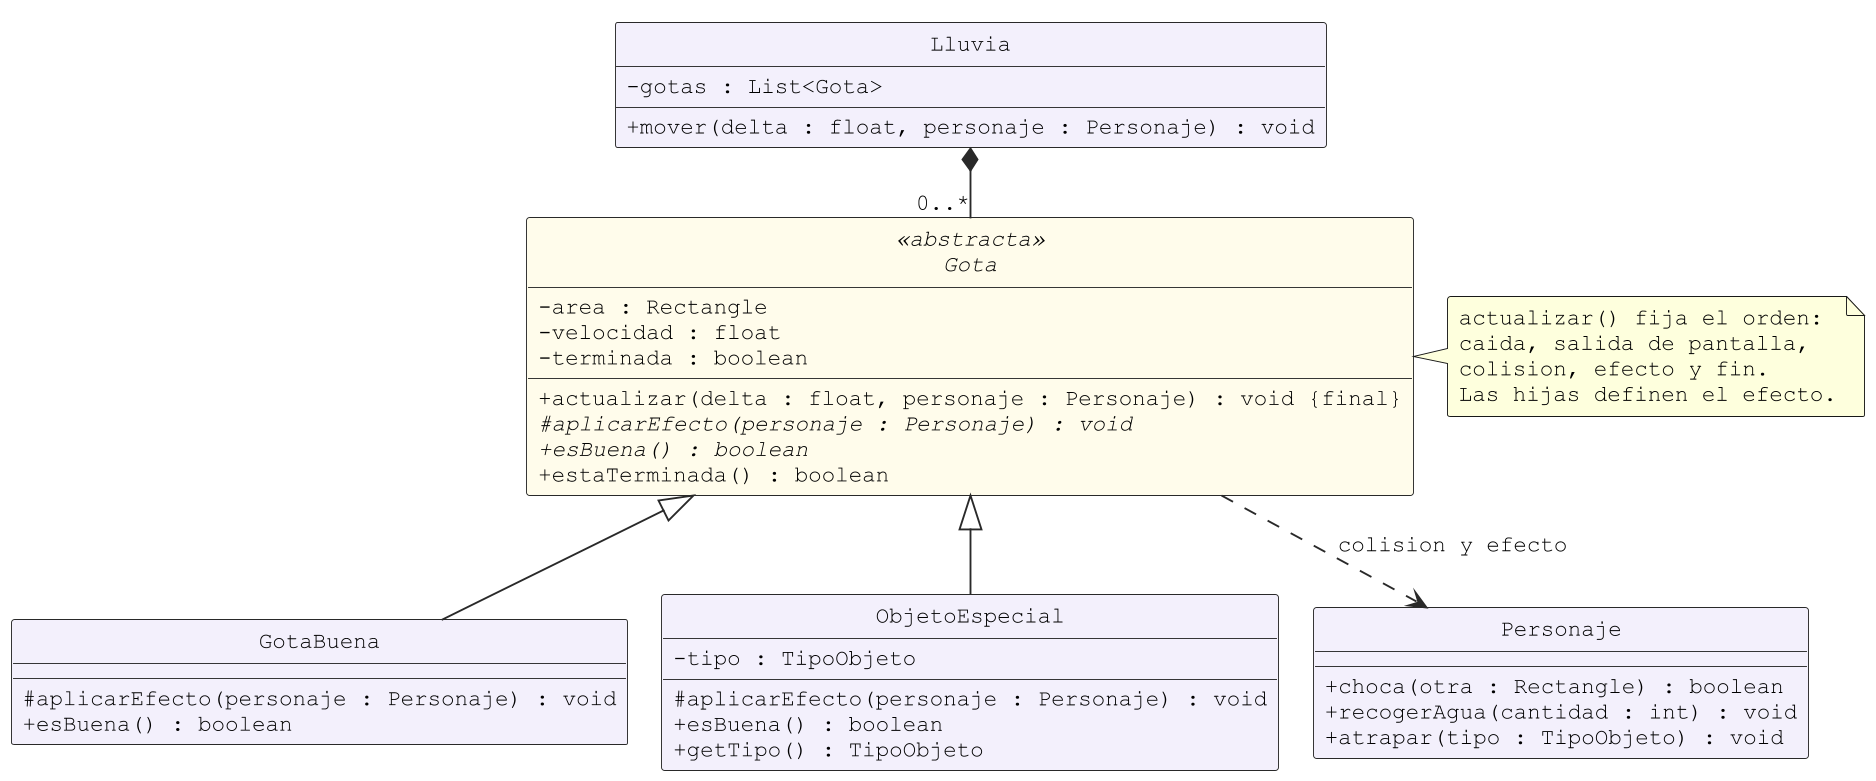
\includegraphics[width=0.95\linewidth,height=0.84\textheight,keepaspectratio]{images/04-template-method.png}
\caption{Template Method en la jerarquía de gotas}
\end{figure}




